\begin{multicols*}{2}

\noindent \textit{М. Волькенштейн}

{\huge \textbf{Квантование}} \\
{\huge \textbf{и стоячие волны}}

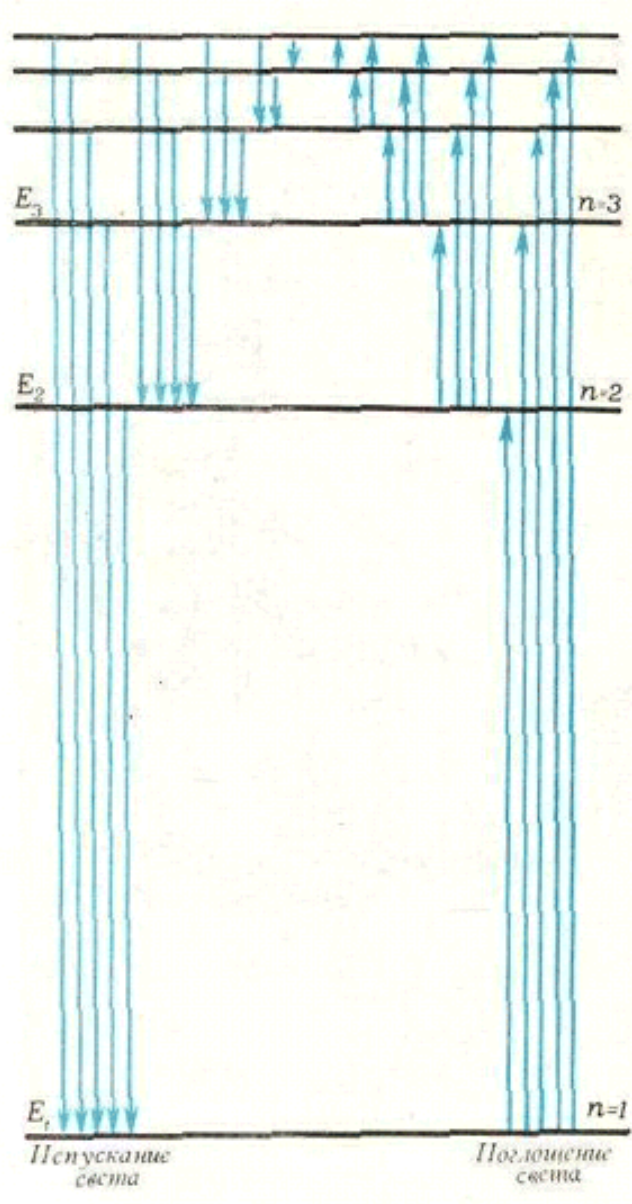
\includegraphics[width=0.9\linewidth, height=20cm]{frontpage.png}

\columnbreak

Квантовая механика — это наука о законах движения микрочастиц (атомов, электронов, нейтронов и т. п.). Это — физика микромира. Она объясняет множество важнейших явлений — и радиоактивный распад, и электропроводность металлов, и природу химической связи. Но прежде всего квантовая механика объяснила линейчатые спектры атомов — ответила на вопрос о том, почему атомы способны испускать или поглощать свет лишь со строго определенными частотами колебаний световой волны. Квантовая механика показала, что электроны в атомах могут обладать только фиксированными, прерывными значениями энергии. Физики обычно говорят, что электроны располагаются на дискретных уровнях энергии $E_1, E_2, \dots$ — энергия электрона в атоме квантована. Поглощение или испускание света атомом происходит при переходе электрона с одного уровня энергии на другой. В первом случае электрон переходит с уровня с меньшей энергией на уровень с большей энергией, во втором случае — наоборот. Частота испускаемой (или поглощаемой) световой волны определяется условием частот Бора.

\vspace{1em}

{\large
\begin{equation}
\nu_{nn'} = \frac{E_n - E_{n'}}{h}, \tag{1}
\end{equation}
}

\noindent где $E_n, E_{n'}$ — уровни энергии, $n, n'$ — значения квантового числа, характеризующего эти уровни.

Одна из главных задач квантовой механики состоит в нахождении квантованных значений энергии для данной системы частиц, в частности, для атома. Согласно уравнению (1) решение такой задачи означает одновременно и расчет спектра системы, то есть определение набора частот света, испускаемого этой системой. Строгое решение этой задачи сводится к решению основного уравнения квантовой механики, так называемого уравнения Шредингера. Это — дифференциальное уравнение в частных про...

\end{multicols*}
